% !TeX spellcheck = en_GB
%\documentclass[handout]{beamer}\mode<presentation>{\usetheme{AMSCesenaPurpleAndGold}}
\documentclass[presentation]{beamer}\mode<presentation>{\usetheme{AMSCesenaPurpleAndGold}}
%%%%

\usepackage{sd-lab-ws}
\usepackage{my-listings}
\usepackage{forloop}

\newcommand{\bs}[1]{\textbackslash{}#1}
\newcommand{\labN}{8}
\newcommand{\labGroup}{https://gitlab.com/pika-lab/courses/ds/ay2021}
\newcommand{\labRepo}{\labGroup/lab-\labN}

\title{L\labN{} -- ReSTful Web Services}
%
\subtitle[SD]{Distributed Systems / Technologies}
%
\author[Ciatto \and Omicini]
{\emph{Giovanni Ciatto} \and Andrea Omicini\\
	\texttt{giovanni.ciatto@unibo.it \and andrea.omicini@unibo.it}}
%
\institute[DISI, Univ. Bologna]
{Dipartimento di Informatica -- Scienza e Ingegneria (DISI)\\\textsc{Alma Mater Studiorum} -- Universit{\`a} di Bologna a Cesena}
%
\date[A.Y. 2020/2021]{Academic Year 2020/2021}

\setbeamercovered{transparent}

\AtBeginSection{
	\begin{frame}[c]\frametitle{Outline}
		% 		\begin{multicols}{2}
		\tableofcontents[sectionstyle=show/shaded, subsectionstyle=hide/hide, subsubsectionstyle=hide/hide]
		% 		\end{multicols}
	\end{frame}
}

\AtBeginSubsection{
	\begin{frame}[c]\frametitle{Next in Line\ldots}
		\begin{multicols}{2}
			\small
			\tableofcontents[sectionstyle=show/shaded, subsectionstyle=show/shaded, subsubsectionstyle=hide/hide]
		\end{multicols}
	\end{frame}
}

\begin{document}

%\\\\\\\\\\\\\\\\\\\\\
\frame{\titlepage}
%\\\\\\\\\\\\\\\\\\\\\

\section{Motivation and Goals}

\begin{frame}[allowframebreaks]
\frametitle{Motivation}

\begin{itemize}
    \item \alert{Web services} are a common pattern for nowadays distributed systems
    %
    \begin{itemize}
        \item Probably, most applications you use every day are web services
        \item[eg] Facebook, Instagram, YouTube, PayPal, Spotify, Netflix, and, yaeh, \alert{Trenitalia} too
    \end{itemize}

    \vspace{.3cm}

    \item Most web services adhere to the \alert{\emph{Re}presentational \emph{S}tate \emph{T}ransfer} (ReST) architectural style, which is the \emph{de facto} standard for web services

    \vspace{.3cm}

    \item This means they expose a \alert{ReSTful API} which is used to wrap a server implemented with some arbitrary technology
    %
    \begin{itemize}
        \item Such an API is usually formalised by means of some \alert{specification language} and it is publicly available

        \item[eg] \href{https://developers.google.com/apis-explorer/\#p/youtube/v3}{YouTube Data API v3}
    \end{itemize}

    \framebreak

    \item Clients -- possibly implemented with some different technology -- can interact with the web service simply by means of such an API

    \vspace{.3cm}

    \item The ReST principles are often reified into a number of good practices aimed at creating \alert{scalable} and \alert{interoperable} systems which are easy to design, develop, and maintain
    %
    \begin{itemize}
        \item[eg] \url{https://www.restapitutorial.com/}
    \end{itemize}
\end{itemize}
\end{frame}

\begin{frame}%[allowframebreaks]
\frametitle{Lecture Goals}
    \begin{itemize}
        \item Recall the Hyper Text Transfer Protocol (HTTP)
        %
        \begin{itemize}
            \item (Even if it is not the only choice, HTTP is usually the base protocol of choice)
        \end{itemize}

        \vfill

        \item Understand how ReST principles are reifyied into good practices and patterns for HTTP-based application

        \vfill

        \item Learn how to produce a (semi-)formal \alert{API specification} by means of de facto standard tools

        \vfill

        \item Learn how a ReSTful \emph{server} should be designed and implemented

        \vfill

        \item Learn how pre-existing, local software gave can be \alert{wrapped} within web services and \alert{distributed}
    \end{itemize}
\end{frame}

\subsection{About the practical activities}

\begin{frame}
\frametitle{Lab \labN{} Repository on GitLab}

	\begin{itemize}
		\item Examples and exercises described in this lecture are provided by means of the following GitLab repository:
		%
		\begin{center}
			\url{\labRepo}
		\end{center}

		\vfill

		\item Clone it on your machine using Git
		%
		\begin{itemize}
		    \item[\$] \texttt{git clone \textit{<repo URL>}}
		\end{itemize}

		\vfill

		\item We kindly suggest to import the cloned repository into some IDE (e.g. IntelliJ Idea or Eclipse) since the volume of the provided code is considerable
		%
		%
		% \begin{itemize}
		%     \item in case of problems in importing the project on IntelliJ, try to downgrade the gradle wrapper
		%     %
		%     \item[\$] \texttt{./gradlew wrapper \alert{--gradle-version \textit{4.8.1}}}
		% \end{itemize}

		\vfill

		\item In order to be able to submit your exercises, please ensure you requested access to the \href{\labGroup}{GitLab group of the course}
	\end{itemize}

\end{frame}


\section{Recall the HTTP protocol}

\subsection{Overview}

\begin{frame}[allowframebreaks]
\frametitle{HTTP Overview}

    \begin{itemize}
        \item One or more \alert{clients} can communicate with a server by means of \alert{synchronous} RPC calls

        \vspace{.3cm}

        \item Each client issues a \alert{request} and waits for a \alert{response} from the server. In any case:
        %
        \begin{itemize}
            \item requests are directed towards an \alert{URL}, i.e. an name for a resource hosted by the server

            \item requests specify a \alert{method}, i.e. an operation with a standard semantics to be performed on the resource

            \item responses carry a \alert{status code} with a standard semantics
        \end{itemize}

        \vspace{.3cm}

        \item Each server is indefinitely \alert{waits} for incoming requests, and, as soon as they arrive, it produces and sends back a response
        %
        \begin{itemize}
            \item in doing, the server may interact with other server or \alert{databases}, behaving as a client w.r.t. them

        \end{itemize}

        \vspace{.3cm}

        \item Requests may possibly provide some \alert{input arguments}, possibly carrying some \alert{return value}

        \vspace{.3cm}

        \item \alert{Input arguments} may be placed in several places within \alert{Requests}:
        %
        \begin{itemize}
            \item[eg] paths
            \item[eg] query parameters
            \item[eg] headers
            \item[eg] bodies
        \end{itemize}

        \vspace{.3cm}

        \item \alert{Return values} may be placed in several places within \alert{Responses}:
        %
        \begin{itemize}
            \item[eg] headers
            \item[eg] bodies
        \end{itemize}
    \end{itemize}

\end{frame}

\subsection{HTTP Messages Structure}

\begin{frame}{The HTTP \textbf{Request} message structure}
    \centering
    \includegraphics[width=\linewidth]{img/http-req.png}
\end{frame}

\begin{frame}{The HTTP \textbf{Response} message structure}
    \centering
    \includegraphics[width=\linewidth]{img/http-res.png}
\end{frame}

\subsection{HTTP Methods}

\begin{frame}{HTTP Methods as CRUD operations}
    \begin{center}
        \includegraphics[width=\linewidth]{img/http-methods.png}
    \end{center}

    \vfill

    \begin{itemize}
        \item CRUD = \emph{C}reate, \emph{R}ead, \emph{U}pdate, \emph{D}elete

        \vfill

        \item Other HTTP methods exist
        %
        \begin{itemize}
            \item[eg] \texttt{TRACE}, \texttt{HEAD}, \texttt{CONNECT}, or \texttt{OPTIONS}
            \item more details are provided at \url{https://www.w3.org/Protocols/rfc2616/rfc2616-sec9.html}
        \end{itemize}
    \end{itemize}
\end{frame}

\subsection{URL Structure}

\begin{frame}{\textbf{Full} structure of URL}
    \begin{center}
        \includegraphics[height=.8\textheight]{img/http-url.png}
    \end{center}
\end{frame}

\begin{frame}{Paths}
    \begin{block}{Paths are usually in the form:}
        \begin{center}
            \texttt{/cathegory/\alert{\{resourceID\}}/subcathegory/\alert{:subResourceID}}
        \end{center}
        %
        where \alert{path parameters} may be denoted through
        %
        \begin{itemize}
            \item curly brackets, e.g. \texttt{\{resourceID\}}
            \item colon, e.g. \texttt{:subResourceID}
        \end{itemize}
    \end{block}

    \begin{exampleblock}{For example, given the parametric URL:}%\small
        \begin{center}
            \texttt{/departments/\alert{\{deptName\}}/professors/\alert{\{profName\}}}
        \end{center}
        one possible instance is:
        \begin{center}
            \texttt{/departments/disi/professors/andrea.omicini}
        \end{center}
        In such case \alert{\texttt{deptName}}=\texttt{disi} and \alert{\texttt{profName}}=\texttt{andrea.omicini}

    \end{exampleblock}

\end{frame}

\begin{frame}[allowframebreaks]{Query parameters}
    \begin{block}{Query parameters are \&-separated key-value pairs in the form:}
        \begin{center}
            \texttt{/path/to/resource \emph{?} \alert{key1}=\textit{value1} \emph{\&} \alert{key2}=\textit{value2} \emph{\&} \ldots}
            \\
            {\tiny{}\alert{(without spaces!)}}
        \end{center}
        %
        where
        %
        \begin{itemize}
            \item the \alert{\texttt{'?'}} char denotes the beginning of the query string
            \item the \alert{\texttt{'\&'}} char separates key-value pairs
            \item the \alert{\texttt{'='}} char separates keys from values
        \end{itemize}
    \end{block}

    \begin{exampleblock}{For example, the query string:}%\small
        \begin{center}
            \texttt{/students\emph{?}\alert{name}=\textit{Giovanni}\emph{\&}\alert{gender}=\textit{male}}
        \end{center}
        carries two sorts of arguments:
        %
        \begin{description}
            \item[\texttt{name}] whose value is \texttt{Giovanni}
            \item[\texttt{gender}] whose value is \texttt{male}
        \end{description}
        %
        and it is a good way to express the query
        %
        \begin{center}
            \textit{select all male students whose name is ``Giovanni''}
        \end{center}
        %
        according to ReST best practices

    \end{exampleblock}
\end{frame}

\begin{frame}{Practical remarks about URLs}

    What if some path/query parameter value contains some URL-reserved character like \texttt{'/'}, \texttt{'?'}, \texttt{'\&'}, \texttt{'\#'} or white spaces?
    %
    \begin{itemize}
        \item path/query arguments must be encoded using the \href{https://en.wikipedia.org/wiki/Percent-encoding}{\alert{Percent-encoding}}
        %
        \begin{itemize}
            \item a.k.a. \alert{URL-encoding}
            \item see also \url{https://en.wikipedia.org/wiki/Percent-encoding}
        \end{itemize}
    \end{itemize}

    \vfill

    \begin{exampleblock}{Example with free text}
    \begin{itemize}
        \item \texttt{Can you read this sentence/phrase?}
        \item \texttt{Can\%20you\%20read\%20this\%20sentence\%2Fphrase\%3F}
    \end{itemize}
    \end{exampleblock}

    \vfill

    \begin{exampleblock}{Example with regular expression}
    \begin{itemize}
        \item \texttt{\textasciicircum{}message \{ content: (.*?) \}\$}
        \item \texttt{\%5Emessage\%20\%7B\%20content\%3A\%20\%28.\%2A\%3F\%29\%20\%7D\%24}
    \end{itemize}
    \end{exampleblock}
\end{frame}

\subsection{Headers}

\begin{frame}{HTTP Headers}
    \begin{itemize}
        \item HTTP headers allow clients and servers to exchange additional information withing the request or the response, in \alert{piggybacking}

        \vfill

        \item The general structure of a HTTP header is a colon-separated pairs:
        %
        \begin{center}
        \begin{tabular}{rlc}
            \texttt{StandardHeader\alert{:}} & \texttt{Value} & {\tiny{}(for standard HTTP headers)}
            \\
            \texttt{\alert{X-}CustomHeader\alert{:}} & \texttt{Value} & {\tiny{}(for user-defined headers)}
        \end{tabular}
        \end{center}

        \vfill

        \item Main headers we will use in this course:
        %
        \begin{description}
            \item[\texttt{Authorization}] | usually present in requests, contains the user credentials, arbitrary encoding
            \item[\texttt{Content-Type}] | usually present in both requests and responses, contains the \alert{MIME-type} of the message body
            \item[\texttt{Accept}] | usually present in requests, contains the \alert{MIME-type(s)} the client is able to understand
        \end{description}
    \end{itemize}
\end{frame}

\subsection{MIME types}

\begin{frame}[allowframebreaks]{MIME types}

    \begin{block}{MIME type}
        The \alert{Multipurpose Internet Mail Extensions} (MIME) type is a de-facto standard way to indicate the nature and format of a document
        %
        \begin{itemize}\small
            \item general structure: \alert{\texttt{type/\textit{subType}}}
        \end{itemize}
    \end{block}

    \framebreak

    \begin{center}
        \includegraphics[width=\linewidth]{img/mime_types.png}
        \small
        (Source: \url{https://developer.mozilla.org/en-US/docs/Web/HTTP/Basics_of_HTTP/MIME_types})
    \end{center}

\end{frame}

\subsection{Message bodies}

\begin{frame}{Message bodies}
    \begin{itemize}
        \item Message bodies carry the \alert{representations} of the resources being manipulated by the client through the server

        \vfill

        \item They usually consist of \alert{textual files} adhering to some particular \alert{schema} (i.e. data type)

        \vfill

        \item Such documents are usually \alert{represented} according to a MIME type
        %
        \begin{itemize}
            \item Most common ones are \texttt{text/\alert{html}}, \texttt{application/\alert{xml}}, \texttt{application/\alert{json}}, and \href{https://en.wikipedia.org/wiki/YAML}{\texttt{application/\alert{yaml}}}
        \end{itemize}

        \vfill

        \item Schemas are usually defined by means of \alert{schema languages}:
        %
        \begin{itemize}
            \item \href{https://www.w3schools.com/xml/schema_intro.asp}{XML Schema} for XML

            \item \href{https://json-schema.org/learn/getting-started-step-by-step.html}{JSON Schema} for JSON or YAML

            \item Some attempts exist to create a (more) target-neutral schema language: \href{https://swagger.io/specification/\#schemaObject}{Open API specification}
        \end{itemize}
    \end{itemize}
\end{frame}


\begin{frame}{Example -- OpenAPI schema for \texttt{User} data type}
    \vspace{-.7cm}
    \begin{columns}[t]
        \begin{column}{.49\textwidth}
            \lstinputlisting[language=yaml]{code/User.yaml}
        \end{column}
        \hfill
        \begin{column}{.49\textwidth}
            \lstinputlisting[language=yaml]{code/UserInstance.yaml}
            \lstinputlisting[language=yaml]{code/UserInstance.json}
        \end{column}
    \end{columns}
\end{frame}

\subsection{Status Codes}

\begin{frame}{HTTP Status Codes -- Overview}
    \includegraphics[width=\linewidth]{img/http_status_codes.png}
\end{frame}

\begin{frame}[allowframebreaks]{HTTP Status Codes -- Ranges}
    \begin{block}{\texttt{1xx} -- Informational}
        \begin{center}
            The request was received, continuing process
        \end{center}
    \end{block}

    \begin{block}{\texttt{2xx} -- Success}
        \begin{center}
            The request was successfully received, and accepted
        \end{center}
        %
        \begin{itemize}
            \item[eg] \alert{\texttt{200 OK}}: Standard response for successful HTTP requests

            \item[eg] \alert{\texttt{204 No Content}}: Like 200 but response contains \alert{no body}
        \end{itemize}
    \end{block}

    \begin{block}{\texttt{3xx} -- Redirection}
        \begin{center}
            Further action are needed to complete the request
        \end{center}
    \end{block}

    \begin{block}{\texttt{4xx} -- Client Error}
        \begin{center}
            The request contains bad syntax or cannot be fulfilled
        \end{center}
        %
        \begin{itemize}
            \item[eg] \alert{\texttt{400 Bad Request}}: The server cannot or will not process the request due to an apparent client error (e.g., malformed request syntax)

            \item[eg] \alert{\texttt{401 Unauthorized}}: Authentication is required and has failed or has not yet been provided

            \item[eg] \alert{\texttt{403 Forbidden}}: Authentication was successful but the client has no permission to perform the requested operation

            \item[eg] \alert{\texttt{409 Conflict}}: Indicates that the request could not be processed because of conflict in the current state of the resource
        \end{itemize}
    \end{block}

    \begin{block}{\texttt{5xx} -- Server Error}
        The server failed to fulfill an apparently valid request
        %
        \begin{itemize}
            \item[eg] \alert{\texttt{500 Internal Server Error}}: A generic error message

            \item[eg] \alert{\texttt{501 Not Implemented}}: The server either does not recognize the request method, or it lacks the ability to fulfil the request
        \end{itemize}
    \end{block}
\end{frame}

\subsection{Routes}

\begin{frame}{Routes}

    \begin{itemize}
        \item The behaviour of WS is designed \& implemented through \alert{routes}

        \vfill

        \item There is no precise definition of what a route is, however the expression roughly refers to some \alert{possible operation} the service may expose to let clients manipulate some \alert{resource}
        %
        \begin{itemize}
            \item[eg] think about a method signature in some Java interface
        \end{itemize}

        \vfill

        \item ``Route'' is usually a \alert{jargon} for:
        %
        \begin{itemize}
            \item[+] an HTTP \alert{method}

            \item[+] a (possibly \emph{parametric}) URL

            \item[+] a set of input arguments, along with their schema, place (URL, body, query, header), and supported MIME types

            \item[+] a set of possible status codes, along with their result types \& MIME type
        \end{itemize}

        \vfill

        \item The service \alert{Web API} consists of the set of its routes declarations

        \vfill

        \item Example of \alert{Web API} \url{https://petstore.swagger.io}
    \end{itemize}

\end{frame}

\section{ReSTful WS Design}

\subsection{Workflow}

\begin{frame}{ReST project design workflow}

When designing a ReST-full web-service, you are encouraged to follow this procedure:
%
\begin{enumerate}
    \item structure your application in terms of \alert{resources} and \alert{sub-resources}

    \vfill

    \item for each (sub-)resource, define a possibly parametric \alert{path}

    \vfill

    \item for each path, define the \alert{methods} it supports, thus defining a \alert{route}

    \vfill

    \item for each route, define:
    %
    \begin{enumerate}
        \item the supported \alert{query parameters} for the request

        \item the supported input \alert{MIME types} and the \alert{schema} of the request body. if any

        \item all the possible results, i.e.:
        %
        \begin{itemize}
            \item all possible \alert{status codes}\ldots

            \item \ldots and the corresponding schemas for the response bodies

        \end{itemize}

        \item optionally, you may also define if \alert{authentication} is required and which sorts of \alert{authorizations} are needed
    \end{enumerate}
\end{enumerate}

\end{frame}

\subsection{OpenAPI Specification}

\begin{frame}{OpenAPI Specification and Swagger}

The design and test phases of a ReST-full web service \alert{API} can be greatly simplified by some (almost) standard technologies:
%
\begin{itemize}
    \item The \alert{OpenAPI Specification} (OAS) is a formal language for describing the API of the service
    %
    \begin{itemize}
        \item Current version of the specification is \href{https://github.com/OAI/OpenAPI-Specification/blob/master/versions/3.1.0.md}{version 3.1.0}, but we will use \href{https://github.com/OAI/OpenAPI-Specification/blob/master/versions/2.0.md}{version 2.0} since it is more mature
    \end{itemize}

    \vfill

    \item In practice, one may actually define a service API by writing a \alert{YAML/JSON file} adhering to the OAS

    \vfill

    \item \href{https://swagger.io}{Swagger} is a community developing and maintaining the OAS, other than a number of useful tools easing the life of API designers and implementors
    %
    \begin{itemize}
        \item \href{https://editor.swagger.io}{Swagger Editor} is a web-based editor for writing specification files

        \item \href{https://swagger.io/tools/swagger-codegen/}{Swagger Codegen} is a tool generating client and server stubs out of an OAS specification file

        \item \href{https://app.swaggerhub.com}{SwaggerHub} is a web repository letting people edit, store, and publish their services APIs
    \end{itemize}

\end{itemize}

\end{frame}

\begin{frame}[allowframebreaks]{Main structure of a OAS specification file}
    \lstinputlisting[language=yaml]{code/SwaggerMain.yaml}
\end{frame}

\begin{frame}[allowframebreaks]{Route definition example}
    \lstinputlisting[language=yaml]{code/RouteExample.yaml}
\end{frame}

\section{HTTP in Practice}

\subsection{Overview}

\begin{frame}{Client- vs. Server-side}

    \begin{itemize}
        \item When working with HTTP, developers rarely implement the protocol from scratch

        \vfill

        \item Conversely, they rely on pre-existing libraries of HTTP-based development

        \vfill

        \item Virtually all languages/platforms provide some library for HTTP
        %
        \begin{itemize}
            \item either via their Standard Library or via third-party libraries
        \end{itemize}

        \vfill

        \item Regardeless of technological details, HTTP libraries are of 2 sorts:
        %
        \begin{description}
            \item[\emph{client}-side] libraries, exposing some means to \alert{issue} HTTP requests towards some server
            \item[\emph{server}-side] libraries, exposing some means to \alert{serve} HTTP requests coming from clients
        \end{description}
    \end{itemize}

\end{frame}

\begin{frame}{HTTP Libraries for Java}

    \begin{itemize}
        \item Java SE is poorly suited for HTTP
        %
        \begin{itemize}
            \item especially for Java $<$ 11
            \item conversely, Java EE is plenty of industry-ready tools for WS
        \end{itemize}

        \vfill

        \item However, the JVM ecosystem is plenty of open-source libraries for HTTP programming

    \end{itemize}

    \vfill

    \begin{block}{JVM technologies for HTTP \textbf{server}-side}
        \href{https://vertx.io}{Vert.X},
        \href{https://javalin.io/}{\emph{Javalin}},
        \href{https://www.playframework.com/}{Play},
        \href{https://javaee.github.io/glassfish/}{Glassfish},
        \href{http://nanohttpd.org}{NanoHTTPd}
    \end{block}

    \vfill

    \begin{block}{JVM technologies for HTTP \textbf{client}-side}
        \href{https://vertx.io}{Vert.X},
        \href{https://docs.oracle.com/en/java/javase/11/docs/api/java.net.http/java/net/http/package-summary.html}{\emph{\texttt{java.net.http.*} (since Java 11)}},
        \href{https://github.com/googleapis/google-http-java-client}{Google HTTP Client Library for Java},
        \href{https://hc.apache.org/}{Apache's HTTP Components},
        \href{https://square.github.io/okhttp/}{OkHttp}
    \end{block}

\end{frame}

\begin{frame}{HTTP Libraries for Java in this Course}
    In this course we focus upon:
    %
    \begin{description}
        \item[\href{https://javalin.io/}{\emph{Javalin}}] for what concerns the \alert{server}-side
        \item[\href{https://docs.oracle.com/en/java/javase/11/docs/api/java.net.http/java/net/http/package-summary.html}{\emph{\texttt{java.net.http.*}}}] for what concerns the \alert{client}-side
        %
        \begin{itemize}
            \item[!] please ensure your JDK is $\geq 11$
        \end{itemize}
    \end{description}

    \vfill

    \begin{block}{Takeaway}
        \begin{itemize}
            \item Despite syntactical differences, server-side HTTP libraries share similar API
            \item A similar argument holds for client-side HTTP libraries
            \item We will try to keep our discussion general
        \end{itemize}
    \end{block}

\end{frame}

\subsection{Client-side Programming}

\begin{frame}%[allowframebreaks]
\frametitle{General Client-side Library}

    You can expect a \emph{client}-side HTTP library to expose these functionalities:
    %
    \begin{itemize}
        \item represent URI/URL

        \vfill

        \item add \emph{query parameters} to URI/URL

        \vfill

        \item URL-encode or decode strings

        \vfill

        \item (de)serialize data (usually in/from XML, \alert{JSON}, or YAML)

        \vfill

        \item build HTTP \emph{requests}, letting developers specify:
        %
        \begin{itemize}
            \item the target URI/URL (possibly including query parameters)
            \item the HTTP \emph{method}
            \item one or more HTTP \emph{headers}
            \item the \emph{body} of the request (out of strings, streams, byte arrays, etc)
        \end{itemize}

        \vfill

        \item handle HTTP responses, possibly \emph{asynchronously} and \emph{concurrently}

        \vfill

        \item configure several low-level protocol aspects
        %
        \begin{itemize}
            \item e.g. timeouts, cookies, cryptographic certificates, etc
        \end{itemize}
    \end{itemize}
\end{frame}

\begin{frame}[allowframebreaks]
    \frametitle{Working tih URL/URI in Java}

    \begin{block}{URL $\subset$ URI (Recap)}
        \begin{description}
            \item[Uniform Resource Identifier (URI)] | string \alert{identifying} a resource
            \item[Uniform Resource Locator (URL)] | string \alert{locating} a resource
        \end{description}
        %
        \begin{itemize}
            \item[$\rightarrow$] all URL are URI, yet not all URI are URL
        \end{itemize}
    \end{block}

    \begin{block}{\texttt{URL} and \texttt{URI} classes in Java}
        \begin{description}
            \item[\href{https://docs.oracle.com/en/java/javase/15/docs/api/java.base/java/net/URL.html}{\texttt{java.net.\textit{URL}}}] | ancient implementation (since Java 1)
            \item[\href{https://docs.oracle.com/en/java/javase/15/docs/api/java.base/java/net/URI.html}{\texttt{java.net.\textit{URI}}}] | novel implementation (since Java 4), RFC compliant
        \end{description}
        %
        \begin{itemize}
            \item when working with web resources the two are quite interchangeable
            \item[!] we will mostly work with the \texttt{URI} class
        \end{itemize}
    \end{block}

    \begin{block}{URI general structure}
        \begin{center}\ttfamily
            [scheme:][//authority][path][?query][\#fragment]
        \end{center}

        \begin{itemize}
            \item[!] When an URI represents an URL:
            %
            \begin{itemize}
                \item scheme $\approx$ protocol
                \item authority $\approx$ domain + port
            \end{itemize}
        \end{itemize}
    \end{block}

    \begin{block}{\texttt{URI} class -- Creation}
        \begin{description}
            \item[\texttt{URI.create(string)}] | parses a string as an URI
            \item[\texttt{new URI(protocol, domain, path, query, fragment)}] | constructs an URI representing an URL, out of 5 strings
        \end{description}
    \end{block}

    \begin{block}{\texttt{URI} class -- Usage}
        Instances of \texttt{URI} are \emph{immutable}, therefore only accessors are available
        %
        \begin{description}
            \item[\texttt{uri.getScheme()}] | gets the scheme, i.e. the \emph{protocol} in case of URL (\texttt{`://'} not included) 
            \item[\texttt{uri.getAuthority()}] | gets the authority (i.e. the \emph{domain} + \emph{port})
            \item[\texttt{uri.getPort()}] | gets just the port as integer
            \item[\texttt{uri.getPath()}] | gets the path (\texttt{`/'} included)  
            \item[\texttt{uri.getQuery()}] | gets the query (\texttt{`?'} not included)  
            \item[\texttt{uri.getFragment()}] | gets the fragment (\texttt{`\#'} not included)   
        \end{description}
    \end{block}

    \begin{exampleblock}{More details and examples}\centering
        \url{https://www.baeldung.com/java-url-vs-uri}
    \end{exampleblock}

\end{frame}

\begin{frame}[allowframebreaks]
\frametitle{Working with Charsets and Encodings in Java}
    \begin{block}{Charset vs. Encoding}
        \begin{description}
            \item[Charset] dictates how bytes are interpreted as chars within strings
            \item[Encoding] rules how to represent byte/char strings using some charset
        \end{description}
    \end{block}

    \begin{examples}{Most notable charsets}
        \begin{itemize}
            \item ASCII \url{https://www.asciitable.it/}
            \item UTF-8 \url{https://www.utf8-chartable.de/}
            \item \alert{UTF-16} \url{https://asecuritysite.com/coding/asc2}
            %
            \begin{itemize}
                \item[!] modern programming languages use UTF-16 for strings
            \end{itemize}
        \end{itemize}
    \end{examples}

    \begin{examples}{Most notable encodings}
        \begin{itemize}
            \item identity (i.e. each character represents itself)
            \item identity + some escape sequences (e.g. \texttt{$\backslash{}$n}, \texttt{$\backslash{}$t}, etc.)
            \item URL/Percent encoding
            \item base64 encoding (\url{https://en.wikipedia.org/wiki/Base64}) 
            \item \ldots
        \end{itemize}
    \end{examples}

    \begin{block}{Standard Charsets in Java}
        Two notable charset-related classes:
        %
        \begin{description}
            \item[\href{https://docs.oracle.com/en/java/javase/15/docs/api/java.base/java/nio/charset/Charset.html}{\texttt{java.nio.charset.\textit{Charset}}}] | represent a charset
            \item[\href{https://docs.oracle.com/en/java/javase/15/docs/api/java.base/java/nio/charset/StandardCharsets.html}{\texttt{java.nio.charset.\textit{StandardCharsets}}}] | contains a number of standard instances of \texttt{Charset}
        \end{description}
    \end{block}

    \begin{block}{URL (Percent) Encoding and Decoding in Java}
        Two notable URL-econding-related classes in Java:
        %
        \begin{description}
            \item[\href{https://docs.oracle.com/en/java/javase/15/docs/api/java.base/java/net/URLEncoder.html}{\texttt{java.net.\textit{URLEncoder}}}] | aimed at encoding strings in percent encoding
            \item[\href{https://docs.oracle.com/en/java/javase/15/docs/api/java.base/java/net/URLDecoder.html}{\texttt{java.net.\textit{URLDecoder}}}] | aimed at decoding percent-encoded strings
        \end{description}

        \medskip

        How to use them:
        %
        \begin{description}
            \item[\texttt{URLEncoder.encode(string, charset)}] | converts \texttt{string} in a URL-encoded string using \texttt{charset}
            \item[\texttt{URLDecoder.decode(string, charset)}] | parses \texttt{string} as a URL-encoded string using \texttt{charset}
        \end{description}
    \end{block}

    \framebreak

    Usage example:
    %
    \lstinputlisting[language=Java,morekeywords={var}]{./code/UrlEncodeExample.java}
\end{frame}

\begin{frame}[allowframebreaks]
    \frametitle{Java 11's \texttt{java.net.http.*} API}

    \begin{block}{General Workflow}
        \begin{enumerate}
            \item Create and configure an \texttt{HttpClient}
            \item Build an \texttt{HttpRequest} via a builder
            \item Send the request via the \texttt{HttpRequest} thorugh the \texttt{HttpClient}
            \item Handle the \texttt{HttpResponse} asynchronously, via \texttt{CompletableFuture}s
        \end{enumerate}
    \end{block}

    \begin{block}{Main abstractions and classes}
        \begin{description}
            \item[\href{https://docs.oracle.com/en/java/javase/15/docs/api/java.net.http/java/net/http/HttpRequest.html}{\texttt{java.net.http.\textit{HttpRequest}}}] | represents to-be-sent requests
            \item[\href{https://docs.oracle.com/en/java/javase/15/docs/api/java.net.http/java/net/http/HttpRequest.Builder.html}{\texttt{java.net.http.HttpRequest.\textit{Builder}}}] | provides builders for requests
            \item[\href{https://docs.oracle.com/en/java/javase/15/docs/api/java.net.http/java/net/http/HttpRequest.BodyPublisher.html}{\texttt{java.net.http.HttpRequest.\textit{BodyPublisher}}}] | fills a request body from some source (String, file, etc)
            \item[\href{https://docs.oracle.com/en/java/javase/15/docs/api/java.net.http/java/net/http/HttpRequest.BodyPublishers.html}{\texttt{java.net.http.HttpRequest.\textit{BodyPublishers}}}] | provides some default \texttt{BodyPublisher} via static methods
            \item[\href{https://docs.oracle.com/en/java/javase/15/docs/api/java.net.http/java/net/http/HttpResponse.html}{\texttt{java.net.http.\textit{HttpResponse}}}] | represents to-be-received responses
            \item[\href{https://docs.oracle.com/en/java/javase/15/docs/api/java.net.http/java/net/http/HttpResponse.BodyHandler.html}{\texttt{java.net.http.HttpResponse.\textit{BodyHandler}}}] | states how the body of a response should be processed
            \item[\href{https://docs.oracle.com/en/java/javase/15/docs/api/java.net.http/java/net/http/HttpResponse.BodyHandlers.html}{\texttt{java.net.http.HttpResponse.\textit{BodyHandlers}}}] | provides a number of default \texttt{BodyHandler}s via static methods
            \item[\href{https://docs.oracle.com/en/java/javase/15/docs/api/java.net.http/java/net/http/HttpClient.html}{\texttt{java.net.http.\textit{HttpClient}}}] | entrypoint used to send requests
        \end{description}
    \end{block}

% \end{frame}

% \begin{frame}[allowframebreaks]
%     \frametitle{Java 11's HTTP API -- Usage}

    Creating a client:
    %
    \lstinputlisting[language=Java,morekeywords={var}]{./code/HttpClient.java}

    \framebreak

    Creating a request:
    %
    \lstinputlisting[language=Java,morekeywords={var}]{./code/HttpRequest.java}
    
    \framebreak

    Other methods exist, one for each HTTP method:
    %
    \begin{description}
        \item[\texttt{reqBuilder.GET()}] | issues a GET request with no body
        \item[\texttt{reqBuilder.PUT(bodyPublisher)}] | issues a PUT request some body
        \item[\texttt{reqBuilder.POST(bodyPublisher)}] | issues a POST request some body
        \item[\texttt{reqBuilder.DELETE()}] | issues a DELETE request with no body   
    \end{description}

    \framebreak

    Creating a request with query parameters:
    %
    \lstinputlisting[language=Java,morekeywords={var}]{./code/HttpRequestWithQuery.java}

    \framebreak

    Handling a response:
    %
    \lstinputlisting[language=Java,morekeywords={var}]{./code/HttpResponse.java}

    \framebreak

    \begin{alertblock}{A few notes about HTTP clients}
        \begin{itemize}
            \item multiple requests can be sent via the same client instance
            \item a new request can be sent even \emph{before} the previuos ones have received a response
        \end{itemize}
    \end{alertblock}

    \bigskip

    \begin{exampleblock}{More details and examples}\centering
        \url{https://openjdk.java.net/groups/net/httpclient/recipes.html}
    \end{exampleblock}

\end{frame}

\subsection{Server-side Programming}

\begin{frame}%[allowframebreaks]
\frametitle{General Server-side Library}

    You can expect a \emph{server}-side HTTP library to expose these functionalities:
    %
    \begin{itemize}
        \item spawn one or more servers, listening on \emph{different ports}

        \vfill

        \item configure one or more \emph{routes} on each server, by specifying:
        %
        \begin{itemize}
            \item the route \emph{method}
            \item the (possibly \emph{parametric}) route \emph{path}
            \item a \emph{callback} to be invoked for each request matching the route
        \end{itemize}
        %
        possibly in a \emph{hierarchical} way

        \vfill

        \item schedule \emph{pre}- or \emph{post}-processing activities on \emph{bunches} of routes
        %
        \begin{itemize}
            \item possibly, via \emph{path templates}
            \item (this is usually achieved via \emph{callbacks} as well)
        \end{itemize}

        \vfill

        \item URL-encode or decode strings \& (de)serialize data

        \vfill

        \item inspect relevant fields of requests, upon reception
        %
        \begin{itemize}
            \item e.g. the actual method, URL, headers, body of the request
        \end{itemize}

        \vfill

        \item build HTTP \emph{responses}, possibly \emph{asynchronously} and \emph{concurrently}
        %
        \begin{itemize}
            \item by specifying their \emph{status code}, body, headers, etc.
        \end{itemize}

        \vfill

        \item configure several low-level protocol aspects
        %
        \begin{itemize}
            \item e.g. timeouts, connections management, cryptographic certificates, etc
        \end{itemize}
    \end{itemize}
\end{frame}

\begin{frame}[allowframebreaks]
    \frametitle{Javalin API}

    \begin{block}{About Javalin (\url{https://javalin.io})}
        \begin{itemize}
            \item Simple library for server-side HTTP programming in Java or Kotlin
            \item Very concise, lightweight, and \alert{didattic}
            \item Approach somewhat similar to NodeJS's \href{https://expressjs.com/it/}{Express}
        \end{itemize}
    \end{block}

    \begin{alertblock}{Quick tutorial syntetised from}
        \url{https://javalin.io/documentation}
    \end{alertblock}

    \framebreak

    Minimal server setup in Javalin:
    %
    \lstinputlisting[language=Java,morekeywords={var}]{./code/Javalin101.java}

    \framebreak

    Setting up routes in Javalin via lambda expressions:
    %
    \lstinputlisting[language=Java,morekeywords={var}]{./code/JavalinRoutes.java}

    \begin{itemize}
        \item where \texttt{HTTP\_METHOD} can be any of:
        %
        \begin{itemize}
            \item[] \texttt{get}, \texttt{post}, \texttt{put}, \texttt{post}, \texttt{delete}, etc.
        \end{itemize}
    \end{itemize}

    \framebreak

    Setting up routes in Javalin via ordinary OOP:
    %
    \lstinputlisting[language=Java,morekeywords={var}]{./code/JavalinRoutesNoLambda.java}

    \framebreak

    \begin{block}{What \textbf{can} one do within routes' callbacks (inspecting the \textbf{request})}
        \begin{description}
            \item[\texttt{ctx.\textit{body}()}] | reads the \emph{request body} as a string 
            \item[\texttt{ctx.\textit{pathParam}(name)}] | gets a \emph{path} parameter by \texttt{name}, as string
            \item[\texttt{ctx.\textit{attribute}(key, object)}] | stores a \texttt{key}-\texttt{object} pair into \texttt{ctx}
            \item[\texttt{ctx.\textit{attribute}(key)}] | retrieves an \texttt{object} given its \texttt{key} from into \texttt{ctx}       
            \item[\texttt{ctx.\textit{contentLength}()}] | gets the length of the request body   
            \item[\texttt{ctx.\textit{contentType}()}] | gets the value of the request \texttt{Content-Type} h.  
            \item[\texttt{ctx.\textit{header}(name)}] | gets the value of some request header by \texttt{name}   
            \item[\texttt{ctx.\textit{url}()}] | gets the request \emph{url}   
            \item[\texttt{ctx.\textit{queryParam}(name)}] | gets the value of a query parameter by \texttt{name}
            \item[\texttt{ctx.\textit{queryParam}(name, default)}] | gets the value of a query parameter by \texttt{name}, or \texttt{default} if missing 
        \end{description}
    \end{block}

    \framebreak

    \begin{block}{What \textbf{can} one do within routes' callbacks (producing a \textbf{response})}
        \begin{description}
            \item[\texttt{ctx.\textit{result}(string)}] | fills the response body with \texttt{string}
            \item[\texttt{ctx.\textit{result}(promise)}] | fills the response body with some \texttt{CompletableFuture} result, as soon as it is available
            \item[\texttt{ctx.\textit{contentType}(mimeType)}] | sets the value of the response \texttt{Content-Type} header  
            \item[\texttt{ctx.\textit{header}(name, value)}] | sets the \texttt{value} of some response header by \texttt{name}
            \item[\texttt{ctx.\textit{status}(code)}] | sets the response status \texttt{code}         
        \end{description}
    \end{block}

    \framebreak

    \begin{block}{What \textbf{can} one do within routes' callbacks (producing \textbf{error} responses)}
        Producing an error response is as simple as \alert{throwing}:
        %
        \begin{description}
            \item[\texttt{new BadRequestResponse(msg)}] | to return a 400 response
            \item[\texttt{new UnauthorizedResponse(msg)}] | to return a 401 response
            \item[\texttt{new ForbiddenResponse(msg)}] | to return a 403 response
            \item[\texttt{new NotFoundResponse(msg)}] | to return a 404 response
            \item[\texttt{new MethodNotAllowedResponse(msg)}] | to return a 405 response
            \item[\texttt{new ConflictResponse(msg)}] | to return a 409 response
            \item[\texttt{new InternalServerErrorResponse(msg)}] | to return a 500 response       
        \end{description}
    \end{block}

    \framebreak

    \begin{block}{What \textbf{should} one do within routes' callbacks}
        \begin{enumerate}
            \item Read, deserialise, and validate the request \alert{input} parameters
            %
            \begin{itemize}
                \item \emph{path}, \emph{query}, and \emph{header} parameters, other than the \emph{body}
                \item[!] deserialise according to the \texttt{Content-Type} header value
                \item[!] throw a new \texttt{BadRequestResponse} if deserialisation/validation fail
            \end{itemize}

            \item \alert{Authenticate} the client, using the value of the \texttt{Authorization} h.
            %
            \begin{itemize}
                \item[!] throw a new \texttt{UnauthorizedResponse} if credentials are missing/invalid
            \end{itemize}
            
            \item Check if the client \alert{is allowed} to perform the requested operation
            %
            \begin{itemize}
                \item[!] throw a new \texttt{ForbiddenResponse} if operation is not allowed
            \end{itemize}

            \item Compute the result, possibly accessing to some data storage
            %
            \begin{itemize}
                \item[!] prefer asynchronous programming whenever possible
            \end{itemize}

            \item \alert{Serialise} output values and return them to the client
            %
            \begin{itemize}
                \item[!] serialise via some \emph{type} contained within the request \texttt{Accept} header  
                \item[!] recall to set the 200 status code, and the \texttt{Content-Type} header
            \end{itemize}
        \end{enumerate}
    \end{block}

    \framebreak

    Example stub:
    %
    \lstinputlisting[language=Java,morekeywords={var}]{./code/JavalinRouteStub.java}
    %
    \begin{itemize}
        \item notice that this is where \alert{(un)marshalling} occurs
        %
        \begin{itemize}
            \item via the \texttt{serialise} and \texttt{deserialise} methods
        \end{itemize}

        \item the actual implementation is within \texttt{computeResultAsync}
    \end{itemize}

    \framebreak

    Factorising common operations with \alert{filters}:
    %
    \lstinputlisting[language=Java,morekeywords={var}]{./code/JavalinFilter.java}
    %
    Use cases:
    %
    \begin{itemize}
        \item intercept common error situations
        \item open common DB connections
        \item etc.
    \end{itemize}

\end{frame}

\subsection{(De)Serialisation}

\begin{frame}%[allowframebreaks]
\frametitle{About (De)Serialisation}

    \begin{itemize}
        \item HTTP server- and client-side libraries rarely include some actual support for (de)serialising data

        \vfill

        \item Generally speaking, a (de)serialisation library exposes some means to
        %
        \begin{itemize}
            \item \emph{serialise} data, i.e. convert  in-memory objects into char/byte sequences

            \item \emph{deserialise} data, i.e. parse chars/bytes back into in-memory object of some \emph{type}
        \end{itemize}

        \vfill

        \item Possibly leveraging some common \emph{data representation format}
        %
        \begin{itemize}
            \item[eg] textual formats such as XML, JSON, YAML
            \item[eg] binary formats such as BSON, XDR, AVRO's, Protobuf's
        \end{itemize}
    \end{itemize}

    \vfill

    \begin{block}{Data representation format $\neq$ Encoding}\small
        \begin{itemize}
            \item (D)Econders just provide a particular means to interpret bytes/chars
            \item (De)Serialisers also provide some means to represent \emph{data structures}

            \item[!] All data-representation formats explicitly or implicitly rely on some encoding
            %
            \begin{itemize}
                \item[eg] most textual data representation formats rely on \texttt{UTF-8} or \texttt{UTF-16}
            \end{itemize}
        \end{itemize}
    \end{block}

\end{frame}

\begin{frame}%[allowframebreaks]
    \frametitle{About (De)Serialisation in Java}

    \begin{itemize}
        \item Java SE is quite well suited for (de)serialisation
        %
        \begin{itemize}
            \item[eg] Java's binary serialization framework (a.k.a. \texttt{ObjectInputStream} \& \texttt{ObjectOutputStream})
            \item[eg] Java's \texttt{javax.xml.*} package
        \end{itemize}

        \vfill

        \item However, the JVM ecosystem is plenty of open-source libraries for JSON / YAML support

    \end{itemize}

    \vfill

    \begin{block}{JVM technologies for (de)serialisation}
        \href{https://github.com/google/gson}{\emph{Gson}},
        \href{https://github.com/FasterXML/jackson}{Jackson},
        \href{https://avro.apache.org/docs/1.10.0/}{Apache Avro},
        \href{https://developers.google.com/protocol-buffers}{Google's Protocol Buffers},
        \href{https://thrift.apache.org/}{Thrift}
    \end{block}
    %
    \begin{itemize}\small
        \item[!] Avro, Thrift, and ProtoBuff are actually full-fledged tools for Middleware development
    \end{itemize}

\end{frame}

\begin{frame}[allowframebreaks]
    \frametitle{General (De)Serialisation Library}

    You can expect a (de)serialisation library to expose these functionalities:
    %
    \bigskip
    %
    \begin{itemize}
        \item \emph{convert} objects of some \emph{type} into strings, according to some format

        \bigskip

        \item \emph{write} objects of some \emph{type} onto output streams, according to some format

        \bigskip

        \item \emph{parse} strings in some format into objects of some type \emph{type}

        \bigskip

        \item \emph{read} input streams, parse them according to some format, outputting objects of some \emph{type}
    \end{itemize}

    \framebreak

    \begin{block}{(De)Serialisation usually involves the construction of an AST}
        \hint{AST = abstract syntax tree}
        \begin{description}
            \item[Serialisation:] in-memory object $\rightarrow$ AST $\rightarrow$ byte/char string
            \item[Deserialisation:] byte/char string $\rightarrow$ AST $\rightarrow$ in-memory object
        \end{description}
        %
        \medskip
        %
        \begin{itemize}
            \item Libraries usually include some \emph{types} to let developers build the AST
            %
            \begin{itemize}
                \item[eg] \texttt{JsonElement} and its subclasses in Gson
                \item[eg] \texttt{JsonNode} and its subclasses in Jackson
            \end{itemize}

            \smallskip

            \item Most libraries are able to read/write several \emph{concrete} syntaxes for the same AST
            \begin{itemize}
                \item[eg] Jackson may read/write XML, JSON, or YAML from a \texttt{JsonNode}
            \end{itemize}

            \smallskip

            \item[!] When the concrete syntax is XML, the AST is a.k.a. \emph{Domain Object Model} (DOM)
        \end{itemize}
    \end{block}
\end{frame}

\begin{frame}%[allowframebreaks]
    \frametitle{(De)Serialisation in Strongly-Typed Languages}

    \begin{itemize}
        \item Serialisation and deserialisation are somewhat \emph{asymmetrical} in OOP libraries

        \vfill

        \item While serialising, libriaries know both:
        %
        \begin{itemize}
            \item the actual type of the in-memory object to be serialised
            \item the target data representation format
        \end{itemize}

        \vfill

        \item While deserialising, libraries only know:
        %
        \begin{itemize}
            \item the actual data representation format of the to-be-parsed string
            \item while the target type the wanna-be in-memory object is unknown
        \end{itemize}

        \vfill

        \item[$\rightarrow$] Developers must always specify the \emph{expected type} upon deserialisation
        %
        \begin{itemize}
            \item subtle technicality with deep implications
        \end{itemize}
    \end{itemize}

\end{frame}

\begin{frame}[allowframebreaks]
    \frametitle{Gson API}

    \begin{block}{Main classes}
        \begin{description}
            \item[\href{https://www.javadoc.io/doc/com.google.code.gson/gson/latest/com.google.gson/com/google/gson/JsonElement.html}{\texttt{com.google.gson.\textit{JsonElement}}}] | root type for data AST
            \item[\href{https://www.javadoc.io/doc/com.google.code.gson/gson/latest/com.google.gson/com/google/gson/Gson.html}{\texttt{com.google.gson.\textit{Gson}}}] | entry point for (de)serialising \texttt{JsonElement}s
        \end{description}
    \end{block}

    \begin{exampleblock}{\texttt{JsonElement} type hierarchy}
        \centering
        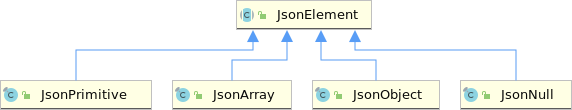
\includegraphics[width=.5\linewidth]{./img/JsonElementCompact.pdf}
    \end{exampleblock}

    \begin{block}{\texttt{Gson} relevant methods}
        \begin{description}
            \item[\texttt{new Gson()}] | creates a new instance of \texttt{Gson}
            \item[\texttt{gson.toJson(jsonElement)}] | generates a JSON string from an AST  
            \item[\texttt{gson.fromJson(string, JsonElement.class)}] | parses an AST out of a JSON string   
        \end{description}
    \end{block}

    \begin{exampleblock}{\texttt{JsonElement} relevant methods}
        \centering
        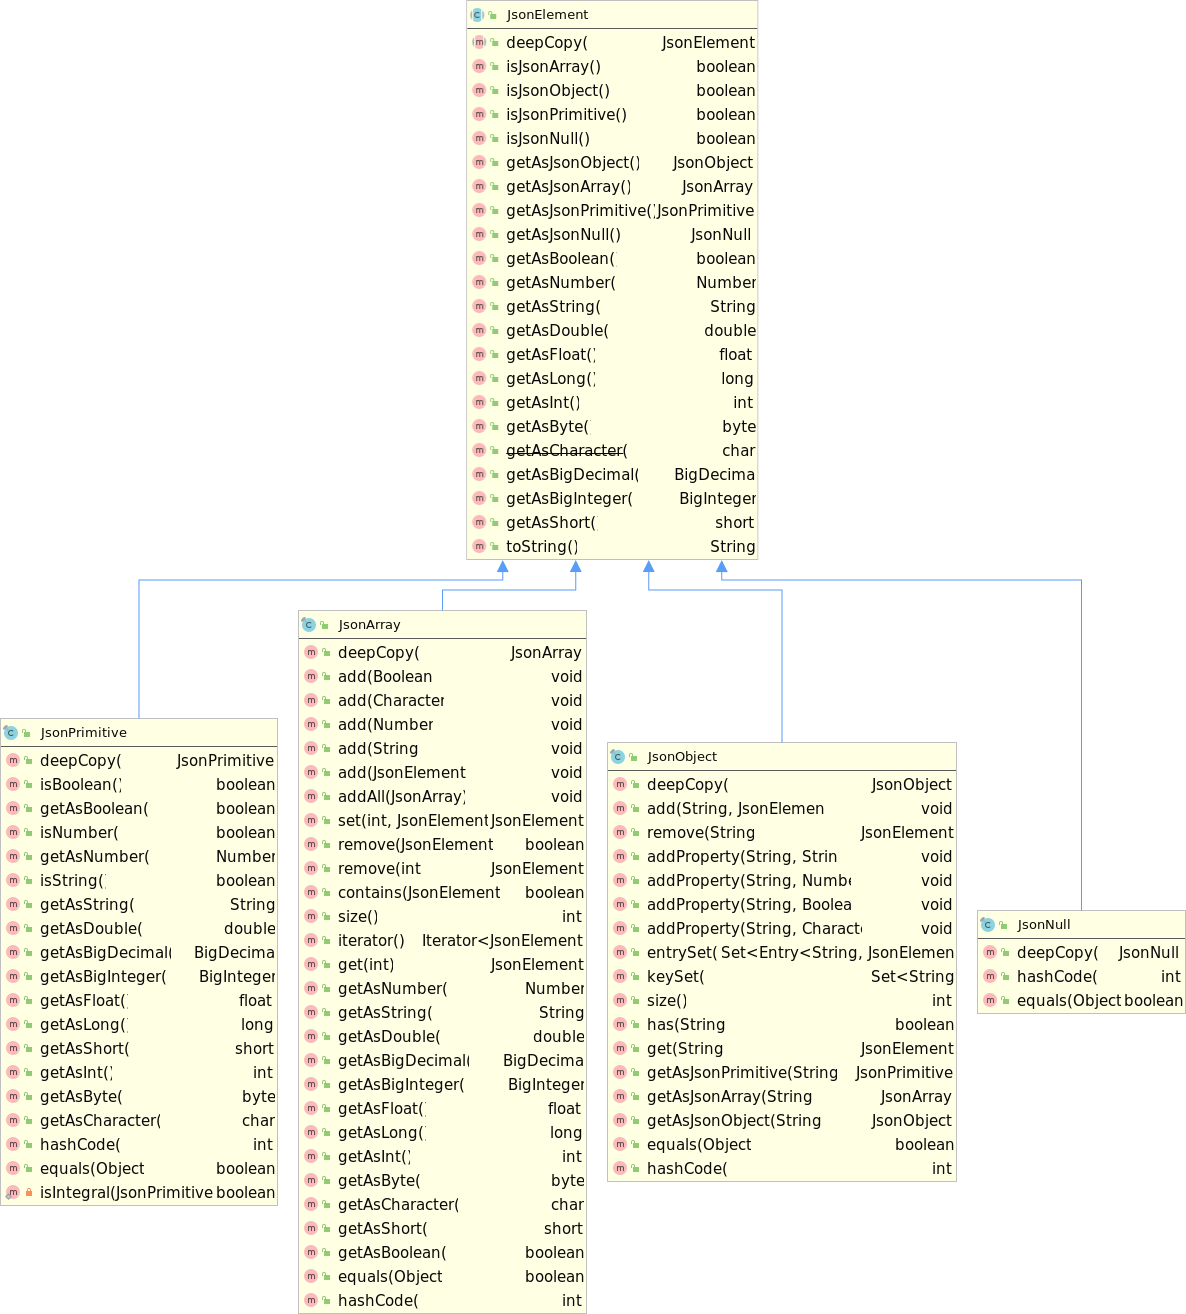
\includegraphics[height=.7\textheight]{./img/JsonElement.pdf}
    \end{exampleblock}

\end{frame}

\begin{frame}[allowframebreaks]
    \frametitle{Gson Example}

    Consider a simple data structure such as:
    %
    \lstinputlisting[language=Java,morekeywords={var}]{./code/Person.java}

    \framebreak

    A serialiser for \texttt{Person}s can be designed as follows:
    %
    \lstinputlisting[language=Java,morekeywords={var}]{./code/PersonSerializer.java}

    \framebreak

    A deserialiser for \texttt{Person}s can be designed as follows:
    %
    \lstinputlisting[language=Java,morekeywords={var}]{./code/PersonDeserializer.java}

\end{frame}

\section{\linda{} Web Service}

\subsection{Overview}

\begin{frame}[allowframebreaks]{Overview}
    \centering
    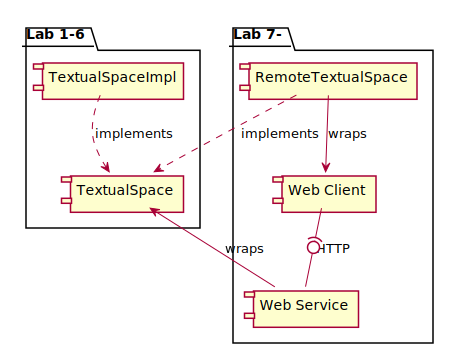
\includegraphics[height=.8\textheight]{img/whole-picture.pdf}

    \bigskip

    \begin{itemize}
        \item In this Lab we will focus on designin \& implementing a \alert{web service} wrapping our \texttt{TextualSpace}s

        \bigskip

        \item This is the first step towards the \alert{distribution} of \linda{} tuple spaces over the network

        \bigskip

        \item After that, we may virtually write a \alert{web client} for any platform, thus bringing \linda{} on other platforms as well

        \bigskip

        \item In that case, distribution could be made \alert{transparent} by wrapping the web client behind the good old local interface
    \end{itemize}
\end{frame}

\subsection{Design}

\begin{frame}[allowframebreaks]{Design of \linda{} WS}
    \begin{itemize}
        \item The design of the \linda{} WS \alert{API} is provided through SwaggerHub
        %
        \begin{center}
            \url{https://app.swaggerhub.com/apis/PIKA-lab/Linda-WS/2}
        \end{center}

        \vspace{.3cm}

        \item The proposed API exposes some routes letting clients access tuple spaces via HTTP
        % \item The proposed API exposes two main groups of routes:
        %
        % \begin{itemize}
        %     \item one (\alert{users}) aimed at supporting clients identities management
        %     \item the other (\alert{tuple-spaces}) aimed at supporting textual spaces and coordination of clients
        % \end{itemize}

        \framebreak

        % \includegraphics[width=\linewidth]{img/ws-api-users.png}

        % \framebreak

        % \item Clients can register themselves using unique usernames, addresses, and passwords
        % %
        % \begin{itemize}
        %     \item Upon registration, they are endowed with an \href{https://it.wikipedia.org/wiki/Universally_unique_identifier}{Universally unique identifier} (UUID)

        %     \item Clients can either be \alert{admins or users}

        %     \item In order to be authenticated, clients must provide their \alert{plain text} credential within the \alert{\texttt{Authorization}} header, in the form
        %     %
        %     \begin{center}
        %         \texttt{\{ "username": "<value>", "password": "value" \}}
        %     \end{center}
        %     Notice that \alert{this is a BAD practice} that we do here just for simplicity

        %     \item \alert{Unauthenticated} clients can interact with the service too, but in a restricted way

        %     \item A logged client can be referenced by means of its username, its address, or its UUID
        %     %
        %     \begin{itemize}
        %         \item i.e. each of these fields can act as an \alert{identifier}
        %     \end{itemize}
        % \end{itemize}

        % \framebreak

        \includegraphics[width=\linewidth]{img/ws-api-tuple-spaces.png}

        \framebreak

        \item Clients may interact by issuing \alert{\linda{} operations} in the form of \alert{HTTP requests} directed towards some textual space wrapped by the service
        %
        \begin{itemize}
            \item textual spaces are referenced through URLs in the form
            %
            \begin{center}
                \texttt{/linda/\alert{v2}/tuple-spaces/\{tupleSpaceName\}}
            \end{center}

            \item tuples are \alert{JSON/YAML files} in the form
            %
            \begin{center}
                \texttt{\{"value": "<string tuple>"\}}
            \end{center}

            \item templates are \alert{query parameters} in the form
            %
            \begin{center}
                \texttt{template=<regex template>}
            \end{center}

            \item primitives are mapped into HTTP methods as follows:
            %
            \begin{center}
                \begin{tabular}{c||c|c|c|c|c}
                    \textbf{Primitive} & \texttt{in} & \texttt{rd} & \texttt{out} & \texttt{get} & \texttt{count}
                    \\
                    \hline
                    \textbf{Method} & \texttt{DELETE} & \texttt{GET} & \texttt{POST} & \texttt{GET} & \texttt{GET}
                \end{tabular}
            \end{center}
        \end{itemize}

        \vspace{.3cm}

        \item Consider reading the API for more details
    \end{itemize}
\end{frame}

\subsection{Implementation}

\begin{frame}{Implementation -- Client-Side vs. Server-Side}

    \begin{itemize}
        \item We cannot ignore distribution any further
        %
        \item The implementation of a WS requires taking care of both
        %
        \begin{itemize}
            \item the \emph{server}-side
            \item the \emph{client}-side
        \end{itemize}
    \end{itemize}

    \vfill

    \begin{block}{The \textbf{server}-side: \texttt{sd.lab.ws.*}}
        \begin{itemize}
            \item providing an HTTP server laveraging Javalin
        \end{itemize}
    \end{block}

    \vfill

    \begin{block}{The \textbf{client}-side: \texttt{{\small sd.lab.linda.textual.impl.}RemoteTupleSpace}}
        \begin{itemize}
            \item providing an implementation of the \texttt{TextualTupleSpace} interface
            \item base on Java 11's \texttt{java.net.http.*} API
        \end{itemize}
    \end{block}

\end{frame}

% \begin{frame}{The \texttt{sd.lab.ws.*} package}

%     The provided code is organised in the many subpackages of \texttt{sd.lab.ws.*}
%     %
%     \vfill
%     %
%     \begin{itemize}

%         \item \alert{\texttt{sd.lab.ws.\textit{presentation}}} contains several classes for the \alert{(un)marshalling} of relevant data types in JSON/XML/YAML

%         \vfill

%         \item \alert{\texttt{sd.lab.ws.\textit{exceptions}}} contains several sorts of \alert{exceptions}, corresponding to as many HTTP errors

%         \vfill

%         \item \alert{\texttt{sd.lab.ws.\textit{storage}}} contains some classes for emulating a \alert{database}
%         storing users or tuple spaces

%         \vfill

%         \item \alert{\texttt{sd.lab.ws.\textit{auth}}} contains some basic \alert{authentication} facilities

%         \vfill

%         \item \alert{\texttt{sd.lab.ws.\textit{routes}}} contains routes implementation \alert{stubs}

%         \vfill

%         \item \alert{\texttt{sd.lab.ws.\textit{api}}} contains routes actual \alert{business logics}
%     \end{itemize}
% \end{frame}

% \begin{frame}{Package \texttt{sd.lab.ws.\textit{presentation}} -- Overview}

%     \centering
%     \includegraphics[width=\linewidth]{img/pkg-presentation.png}

% \end{frame}

% \begin{frame}{Package \texttt{sd.lab.ws.\textit{exceptions}} -- Overview}

%     \centering
%     \includegraphics[width=\linewidth]{img/pkg-exceptions.png}

% \end{frame}

% \begin{frame}{Package \texttt{sd.lab.ws.\textit{storage}} -- Overview}

%     \centering
%     \includegraphics[width=.7\linewidth]{img/pkg-storage.png}

% \end{frame}

% \begin{frame}{Package \texttt{sd.lab.ws.\textit{routes}} -- Overview}

%     \centering
%     \includegraphics[width=\linewidth]{img/pkg-routes.png}

% \end{frame}

% \begin{frame}{Package \texttt{sd.lab.ws.\textit{api}} -- Overview}

%     \centering
%     \includegraphics[width=\linewidth]{img/pkg-api.png}

% \end{frame}

% \begin{frame}{Main class \texttt{sd.lab.ws.\textit{Service}} -- Overview}

%     \centering
%     \includegraphics[width=.5\linewidth]{img/Service.png}

% \end{frame}

% \begin{frame}{Dynamic Structure of Paths and Routes}

%     \texttt{Service}
%     \begin{itemize}
%         \item \texttt{LindaPath}
%         %
%         \begin{itemize}
%             \item \texttt{TupleSpacePath}
%             %
%             \begin{itemize}
%                 \item \texttt{GET /users}
%                 \item \texttt{POST /users}
%                 \item \texttt{GET /users/\textit{\{identifier\}}}
%                 \item \texttt{PUT /users/\textit{\{identifier\}}}
%             \end{itemize}
%             \item \texttt{UsersPath}
%             %
%             \begin{itemize}
%                 \item \texttt{GET /tuple-spaces}
%                 \item \texttt{GET /tuple-spaces/\textit{\{tupleSpaceName\}}}
%                 \item \texttt{POST /tuple-spaces/\textit{\{tupleSpaceName\}}}
%                 \item \texttt{DELETE /tuple-spaces/\textit{\{tupleSpaceName\}}}
%             \end{itemize}
%         \end{itemize}
%     \end{itemize}

% \end{frame}

% \section{Exercises}

% \begin{frame}{Exercise 7-0 -- Understanding}
%     \begin{enumerate}
%         \item Understand the \linda{} WS API on SwaggerHub
%         %
%         \begin{center}
%             \url{https://app.swaggerhub.com/apis/PIKA-lab/Linda-WS/1}
%         \end{center}

%         \vfill

%         \item Understand the structure of the provided code, by navigating it

%         \vfill

%         \item Localise the many TODO into the code

%     \end{enumerate}
% \end{frame}

% \begin{frame}{Exercise 7-1 -- Work with resources}
%     \begin{enumerate}
%         \item Let's focus on the \texttt{"users"} group of routes

%         \vfill

%         \item Have a look to the \texttt{UsersPath} class and the \alert{UsersApi} interface
%         %
%         \begin{itemize}
%             \item Can you understand the meaning \& purpose of each one?
%             \item Can you understand what a \alert{stub} is?
%         \end{itemize}

%         \vfill

%         \item Localise the many TODO into the code

%         \vfill

%         \item Fill the TODOs with your solution

%         \vfill

%         \item Your solution is correct if tests in suit \texttt{TestUsers} succeed

%     \end{enumerate}
% \end{frame}

% \begin{frame}{Exercise 7-2 -- Wrap tuple spaces}
%     \begin{enumerate}
%         \item Let's focus on the \texttt{"tuple-spaces"} group of routes

%         \vfill

%         \item Have a look to the \texttt{TupleSpacePath} class and the \alert{TupleSpaceApi} interface
%         %
%         \begin{itemize}
%             \item Can you understand the meaning \& purpose of each one?
%         \end{itemize}

%         \vfill

%         \item Localise the many TODO into the code

%         \vfill

%         \item Fill the TODOs with your solution
%         %
%         \begin{itemize}
%             \item this time you are required to set up routes and reason on how to implement the ReST API
%         \end{itemize}

%         \vfill

%         \item Tests are a work in progress :)

%     \end{enumerate}
% \end{frame}

%===============================================================================
\section*{}
%===============================================================================

%\\\\\\\\\\\\\\\\\\\\\
\frame{\titlepage}
%\\\\\\\\\\\\\\\\\\\\\

%%===============================================================================
%\section*{\refname}
%%===============================================================================
%
%%\\\\\\\\\\\\\\\\\\\\\
%%%%%
%%\begin{frame}[t,allowframebreaks]\scriptsize
%\begin{frame}[c]\footnotesize
%\frametitle{\refname}
%\bibliographystyle{apalike}
%\bibliography{sd-lab-jadelike-agents}
%\end{frame}
%%\\\\\\\\\\\\\\\\\\\\\

%%%%%%%%%%%%%%%%%%%%%%%%%%%%%%%%%%%%%%%%%%%%%%%%%%%%%%%%%%%%%%%%%%%%%%%%%%%%%%%
\end{document}
%%%%%%%%%%%%%%%%%%%%%%%%%%%%%%%%%%%%%%%%%%%%%%%%%%%%%%%%%%%%%%%%%%%%%%%%%%%%%%%%

